
\begin{frame}% первый слайд
	\titlepage
\end{frame}

\begin{frame}	
	\begin{figure}[h!]
		\centering
		\begin{subfigure}[b]{0.4\linewidth}
			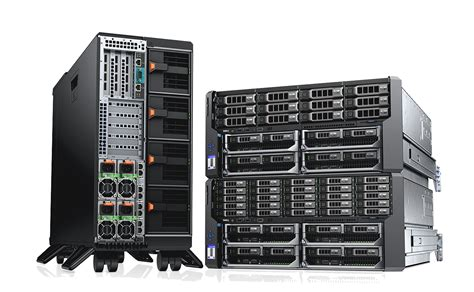
\includegraphics[width=\linewidth]{images/server.jpg}
			\caption{Серверы.}
		\end{subfigure}
		\hfill
		\begin{subfigure}[b]{0.4\linewidth}
			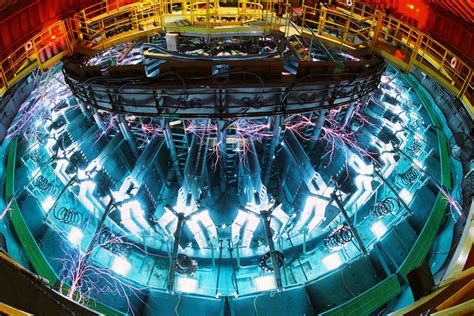
\includegraphics[width=\linewidth]{images/accelerator.jpg}
			\caption{Ускорители.}
		\end{subfigure}
	\end{figure}
	\par
	Существует множество задач, в которых необходимо обрабатывать много независимых событий.
\end{frame}


\begin{frame}{Сопрограммы}
	\begin{itemize}
		\item \textbf{Сопрограмма} (c англ. coroutine) - программный модуль, организованный для обеспечения взаимодействия с другими модулями по принципу кооперативной многозадачности.
		
		\item Сопрограммы способны приостанавливать свое выполнение, сохраняя \textit{контекст} 
		(программный стек и регистры), и передавать управление другой.
	\end{itemize}
\end{frame}

\begin{frame}{Ключевые отличия от потоков ОС}
	Плюсы сопрограмм
	\begin{itemize}
		\item Переключение контекста сопрограммы требует меньше накладных расходов, чем потока.
		\item Как правило меньший размер стека, а значит, потребление памяти так же меньше.
	\end{itemize}

	Минусы
	\begin{itemize}
		\item Сопрограммы не способны исполняться параллельно.
	\end{itemize}
\end{frame}

\begin{frame}{Поддержка в языках программирования}
	
	\begin{figure}
	\centering
	\hfill
	\begin{subfigure}[b]{0.25\linewidth}
		
\includegraphics[width=\linewidth]{images/cpp.png}
		\caption{С++20.}
	\end{subfigure}
	\hfill
	\begin{subfigure}[b]{0.30\linewidth}
		
\includegraphics[width=\linewidth]{images/csharp.jpg} 
		\caption{С\#.}
	\end{subfigure}
	\hfill
	\begin{subfigure}[b]{0.30\linewidth}
		
\includegraphics[width=\linewidth]{images/go.jpg}
		\caption{Go.}
	\end{subfigure}
	
	\end{figure}
	\par
	В языке Java сопрограммы не реализованы.
\end{frame}

\begin{frame}
	
\includegraphics[scale=0.5]{images/loom.jpg}
	
	\begin{itemize}
	\item	Project Loom – проект на базе OpenJDK, целью которого является разработка сопрограмм для языка Java. 
	\item	На данный момент уже доступна ранняя версия проекта.
	\end{itemize}
\end{frame}

\begin{frame}{Цели и задачи}
	
	Цель: реализация прототипа сопрограмм в Java.
	\par
	Поставленные задачи:
	\begin{itemize}
		\item Разработать тесты для сравнения производительности потоков и сопрограмм.
		\item Реализовать переключение сопрограмм.
		\item Реализовать трассировку ссылок объектов на стеках сопрограмм для сборки мусора.
		\item Сравнить производительности сопрограмм и потоков. 
	\end{itemize}

	Работа проводится на базе Huawei JDK.
\end{frame}

\begin{frame}{Тесты производительности}
	Был создан набор тестов на производительность сопрограмм для языков Go, Java (с “Loom Project”).
	
	Тесты создавались для измерения 2 параметров.
	\begin{itemize}
		\item Скорость переключения контекста.
		\item Потребление памяти.
	\end{itemize}
	Репозиторий с тестами: https://github.com/minium2/coroutines-benchmark
	
\end{frame}

\begin{frame}{Переключение сопрограмм}
	\begin{figure}
		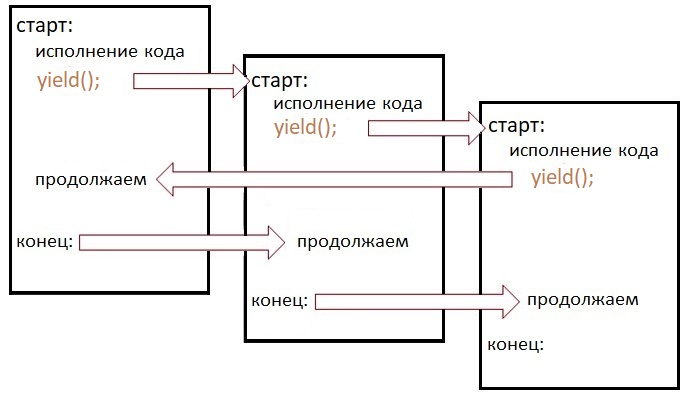
\includegraphics[scale=0.5]{images/scheme.jpg}
	\end{figure}
	\par
	Подходы к реализации:
	\begin{itemize}
		\item OpenJDK(Проект "Loom"): копирование стека сопрограммы при переключении.
		\item Go и HuaweiJDK: изменение указателя стека.
	\end{itemize}
\end{frame}

\begin{frame}{Трассировка стеков}
	\begin{figure}
		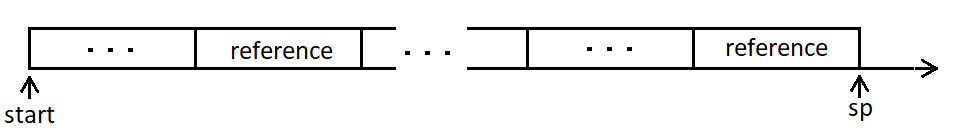
\includegraphics[scale=0.5]{images/stack.png}
	\end{figure}

	\begin{itemize}
		\item Для работы сборщика мусора необходимо найти ссылки на стеке.
		\item Поиск проходит путем итерации значений на стеке и проверка, что они являются ссылками.
	\end{itemize}
\end{frame}	
	
\begin{frame}{Результаты}
	\begin{itemize}
		\item Создан набор тестов для сравнения производительности потоков и сопрограммаами.
		\item Реализовано переключение контекста сопрограмм.
		\item Разработана трассировка ссылок объектов на стеках сопрограмм.
		\item Получены результаты тестов производительности.
	\end{itemize}
\end{frame}

\begin{frame}{Результаты: скорости переключения потоков и сопрограмм}
	Ubuntu, Intel Core i7-8700, 31 Гб ОЗУ, HuaweiJDK
	\par Каждое значение усреднено по 100 измерениям. 
	\par Для измерения используется только одно ядро ЦП.
	\begin{table}[H]
		%\caption{Число переключений корутин}\label{inc-matrix}
		\begin{tabular}{|c|c|c|c|c|c|}
			\hline \multirow{2}{*}{Количество(???), шт.} & \multicolumn{2}{|c|}{Число переключений, 1/сек.}    \\
			\cline{2-3}    & Сопрограммы            & Потоки                  \\
			\hline 100     & 1'246'756 (-/+ 12'961) & 2'306'346 (-/+ 49'831)  \\
			\hline 1'000   & 1'199'142 (-/+ 11'803) & 2'300'279 (-/+ 27'180)  \\
			\hline 5'000   & 1'075'559 (-/+ 59'328) & 1'553'872 (-/+ 36'832)  \\
			\hline 10'000  & 1'016'802 (-/+ 9'990)  & 1'015'976 (-/+ 29'096)  \\ 
			\hline 50'000  & 756'523 (-/+ 8'232)    & 361'088 (-/+ 7'853)     \\ 
			\hline 
		\end{tabular}
	\end{table}
	
\end{frame}


\begin{frame}{Результаты: скорости переключения сопрограмм в управляемых средах}
	Ubuntu, Intel Core i7-8700, 31 Гб ОЗУ, HuaweiJDK
	\par Каждое значение усреднено по 100 измерениям. 
	\par Для измерения используется только одно ядро ЦП.
	
	\begin{table}[H]
		%\caption{Число переключений корутин}\label{inc-matrix}
		\begin{tabular}{|c|c|c|c|c|c|}
			\hline \multirow{2}{*}{шт.} & \multicolumn{3}{|c|}{Число переключений, 1/сек.}      \\
			\cline{2-4}    & HuaweiJDK              & OpenJDK("Loom Project") & Go                     \\
			\hline 100     & 1'246'756 (-/+12'961) & 1'900'009 (-/+19'732)    & 18'187'799 (-/+219367)    \\
			\hline 1000    & 1'199'142 (-/+11'803) & 1'775'239 (-/+20'491)    & 17'934'078 (-/+332778)    \\
			\hline 5000    & 1'075'559 (-/+59'328) & 1'703'631 (-/+30'498)    & 12'892'417 (-/+339410)    \\ % 
			\hline 10000   & 1'016'802 (-/+9'990)  & 1'924'971 (-/+234'982)   & 8'307'791 (-/+79652)     \\ % 
			\hline 50000   & 756'523 (-/+8'232)    & 1'518'349 (-/+152'899)   & 5'292'780 (-/+121844)    \\ % 
			\hline 
		\end{tabular}
	\end{table}	
	
\end{frame}


\begin{frame}{Результаты: потребление памяти}
	Ubuntu, Intel Core i7-8700, 31 Гб ОЗУ
	\begin{table}[H]
		%\caption{Число переключений корутин}\label{inc-matrix}
		\begin{tabular}{|c|c|c|c|c|c|}
			\hline \multirow{2}{*}{Количество(???), шт.} & \multicolumn{3}{|c|}{Размер физической памяти}  \\
			\cline{2-4}    & HuaweiJDK  & OpenJDK   & Go      \\
			\hline 100     & 18 Mб       & 130 Mб     & 3040 Kб  \\
			\hline 1000    & 23 Mб       & 161 Mб     & 3105 Kб  \\
			\hline 5000    & 30 Mб       & 187 Mб     & 3156 Kб  \\
			\hline 10000   & 35 Mб       & 193 Mб     & 3308 Kб  \\
			\hline 50000   & 55 Mб       & 202 Mб     & 3407 Kб  \\ 
			\hline 
		\end{tabular}
	\end{table}
\end{frame}

\begin{frame}{Результаты: потребление памяти}
	Ubuntu, Intel Core i7-8700, 31 Гб ОЗУ, HuaweiJDK
	\begin{table}[H]
		%\caption{Число переключений корутин}\label{inc-matrix}
		\begin{tabular}{|c|c|c|c|c|c|}
			\hline \multirow{2}{*}{Количество, шт.} & \multicolumn{2}{|c|}{Размер физической памяти}  \\
			\cline{2-3}    & Сопрограммы  & Потоки   \\
			\hline 100     & 18 Mб         & 34 Mб     \\
			\hline 1000    & 23 Mб         & 35 Mб     \\
			\hline 5000    & 30 Mб         & 37 Mб     \\
			\hline 10000   & 35 Mб         & 40 Mб     \\
			\hline 50000   & 55 Mб         & 72 Mб     \\ 
			\hline 
		\end{tabular}
	\end{table}
\end{frame}

\begin{frame}{План дальнейших работ} 
	\begin{itemize}
		\item Переделать функцию переключения контекста.
		\item Реализация возможности миграции сопрограмм с одного потока на другой(???).
		\item Синхронизация: поддержка synchronized блоков(???).
		\item Переключение сопрограммы при вызове ввода вывода.
	\end{itemize}
\end{frame}

\begin{frame}
	\begin{center}
		Спасибо за внимание!
	\end{center}
\end{frame}

